
\documentclass[article,pdftex,10pt,a4paper,twocolumn]{article}
\usepackage[authoryear]{natbib}
\usepackage{graphics}

\usepackage{url}\urlstyle{rm}
\usepackage{epstopdf}
\usepackage{graphicx}


\RequirePackage{color}
\def\imagei{\centerline{\color[gray]{.75}\rule{\hsize}{4pc}}}%
\def\imageii{\centerline{\color[gray]{.75}\rule{4pc}{4pc}}}%





\begin{document}


\title{The Detection of Phishing Emails: Feature Selection and Outlier Detection}

\author{Saloni Parkash, Sierra Hawbaker, \\ \small Kansas State University, Manhattan, KS 66502 \\ \small saloni@ksu.edu, sierrahawbaker@ksu.edu}


\maketitle

\begin{abstract}
With this project we have tried to recognize the pattern of emails belonging to phishing and legitimate. It was surprising for us that the language of both types of emails was almost the same, yet there is a different pattern that can be traced with minute observations.  We have, with our project, tried to trace those patterns. So, the goal here is to trace the patterns of both types of emails - what kind of words make these emails really different. We have also tried to discuss the outliers - and with that  method we have tried to detect the novelty with both types of emails. We hope that with this project we can raise the flags to recognize  the phishing emails by the language and pattern.
\end{abstract}


\section{Introduction}
\label{introduction}

%The introduction section should include the following: \newline
%a. Description of the problem or scientific question that is being addressed, and an explanation of why it is important to solve it. \newline
%b. A summary of previous work that was done in the field. This should include references to papers published previously that describe solutions to the same or similar problems. These papers should also be listed in the References section.

%References should be used with the APA format. That can be done easily by using Bibtex with the apalike bibliography style. A reference to a bibliographic source in the text can be done using \cite{ozsvath2001approaches} or \citep{ellis1979homogeneity}.

%If the name of the author of the paper is part of the sentence, the reference should be: \cite{ozsvath2001approaches} proposed a different cosmological model based on a rotating universe.

%If the name of the author is not part of the sentence, the reference should be. In addition to the standard cosmological models, alternative cosmological models were proposed \citep{ozsvath2001approaches}.

%A reference to more than one source can be done by \citep{ozsvath1962finite,godel1949example}.

%The introduction section is a mandatory section that all papers must include. The rest of the paper can include different sections, but the following format is normally effective for data science papers.

In today’s digital world, the threat of phishing emails evolves faster than many security measures. While they often appear indistinguishable from legitimate messages, subtle cues in language and structure can reveal their true intent. Detecting these hidden signals is not just about technology—it’s about understanding how language can be manipulated to deceive. By uncovering these patterns, we can move from reactive defenses to proactive identification, empowering users to recognize threats before damage occurs. This approach offers a new perspective on email security, bridging linguistic insight with cybersecurity strategy.

Phishing emails are a malicious and a common attack vector for actors looking to gain access and information to systems. These types of attacks are effective because they mimic the communication a target commonly interacts with.

Whether the attacker impersonates a higher up, masquerades as a government body, or claims to be an urgent opportunity, the attacker relies on deception. By its nature, deception seeks to remain unnoticed.

Unveiling this deception is a boon because it undermines the key tool these types of attacks use to dupe targets. If the delineation between phishing emails and regular emails is defined, they can be filtered from view of potential targets. If a target does not see a phishing email, they are much less likely to become a victim to the attack.

Phishing emails target human users, as such, they are built to fool human observers. The advantage of a machine learning approach is that it does not rely on human intuition. A machine learning approach may be able to uncover distinctions between the types of emails that are not readily apparent to the either the target of an attack, or the human researcher.

Phishing detection has been an area of interest for researchers in the past. However, since cybersecurity attacks are cat and mouse games between researchers and attackers, there is always room to improve. Beyond prediction, our goal is to recognize similarities and differences between legitimate and phishing emails.

Given the widespread use of email, and the need for sensitive information to remain private, it is no surprise that the detection of phishing emails is not a new target for machine learning applications.

This prior research includes recommendation for the implementation of transformer models. These methods were effective, but widescale application remained a potential issue \citep{alhuzali}. Others considered feature extraction paired with support vector classifiers and natural language processing. Similarly, the ability for large scale application remained an issue \citep{alkhodhairy}.

Many of the recent developments in phishing email detection include or focus on deep learning. This makes sense given the current prevalence of artificial intelligence and deep learning as a whole.

\section{Data}
\label{data}

%In this section you need to describe your data. The description should include the following: \newline
%a. The source of the data, including references when relevant. If the data was collected through an automatic or manual process of data collection that part should also be described. \newline
%b. The size of the data. \newline
%c. Basic description of the data. The description includes classes, distribution of the data by the different classes or by other measurements. The description should include graphs that visualize the distribution of the data, giving the reader more information about the nature of your initial data.\newline
%d. Description of the process of preparing the data for processing. \newline

%Your data section should include tables and/or figures. A simple table can be formatted as follows:


%\begin{table}
%{
%%\footnotesize
%\scriptsize
%\begin{tabular}{|l|c|c|c|c|}
%\hline
%Column 1 &  Column 2    &  Column 3  & Column 4 & Column 5 \\
%\hline
%0   &    9,655   &   64,092  &  10,862     &    84,609    \\
%0.05 &   14,746  &  104,339   & 21,098   &   140,183    \\
%0.1 &    12,142  &  67,712  &  13,797   &    93,651    \\
%0.15  &  7,757    & 33,957  &  8,360     &     50,074    \\
%$>$0.2  &  47,456    & 134,706    & 36,473    &   218,635    \\
%\hline
%Total      &  91,965 &  406,185  & 90,899   & 589,049  \\
%\hline
%\end{tabular}
%\caption{Each table must have a caption.}
%\label{table_label}
%}
%\end{table}


%A simple figure can be formatted using the following syntax. You can use several image formats such as eps or jpeg, but pdf is preferred.

%\begin{figure*}[h]
%\includegraphics[scale=1.0]{figure_file.pdf}
%\caption{Each figure must have a caption}
%\label{figure_label}
%\end{figure*}



%Each table and each figure must also be referenced from the text. For instance, Table~\ref{table_label} shows the data ......
 
Our sources contained both phishing and legitimate emails. Our data came from three sources, the Enron dataset of corporate emails \citep{cohen} and the Ling dataset of emails \citep{sakkis} were both sources of legitimate emails. Together, these datasets contained over five-hundred thousand emails. The third dataset, a set of emails generated by artificial intelligence, contained phishing emails. This data set contained 865 phishing emails \citep{shamir}.

The distribution of legitimate emails to phishing emails was unbalanced. The over representation of legitimate emails in the dataset motivated us to take a random sample of the two sources of legitimate emails and use that subset of the legitimate email data. one-thousand entries from each source were randomly sampled in order to create this subset of the legitimate email data.

However, once vectorized through udat, the final dataset contained 1991 legitimate emails and 865 phishing emails. This is because some emails were skipped due to extremely short length. Udat provided the feature set used with the data in its csv and fit output format.

When required, the data was standardized for analysis as shown in Figure~\ref{3ddistributionofemails}.

\begin{figure}[h]

\includegraphics[scale=0.2]{imgs/data_1}
\caption{3D Distribution of Email Classes}
\label{3ddistributionofemails}
\end{figure}

\newpage
\section{Methods}
\label{methods}

% This section should describe in details the methods that you developed and/or used. A method can be a certain existing software tool that you used, an equation, an algorithm, etc’.  If you used existing methods, a reference to the papers that describe the methods is required.

\subsection{Feature Selection}
\label{methodfeatureselection}

\subsubsection{Feature Selection and Data Preparation}
\label{methodsfeatureselectionanddatapreparation}

We began by cleaning the dataset: missing values were imputed using mean values, and class labels were numerically encoded (phishing = 0, legitimate = 1). Non-informative features such as file path identifiers were removed. To identify relevant features, we computed the mean values for phishing and legitimate emails separately and performed independent two-sample t-tests to assess statistical significance. Features were ranked based on mean differences and p-values, with the top 20 selected for further analysis.

\subsubsection{Classification Models and Evaluation}
\label{methodsclassificationmodelsandevaluation}

Using the selected features, we trained multiple classifiers including Decision Tree, Logistic Regression, AdaBoost, Random Forest, Gradient Boosting, K-Nearest Neighbors, SVM variants, Gaussian Naive Bayes, Linear Discriminant Analysis (LDA), and Quadratic Discriminant Analysis (QDA). The dataset was shuffled and split into training (70\%) and testing (30\%) sets with stratification to maintain class balance. Linear models were trained on standardized features (z-score scaling), while tree-based models used unscaled features due to their scale invariance. Performance metrics included accuracy, sensitivity (true positive rate), and specificity (true negative rate).

\subsubsection{Feature Importance Analysis}
\label{methodsfeatureimportanceanalysis}

Feature importance was extracted from tree-based classifiers via their inherent importance scores, and from Logistic Regression using absolute coefficient values, preserving coefficient signs to indicate feature association direction. For each model, the top 10 features were identified and combined to determine the most frequently selected attributes across classifiers.

\subsubsection{Model Robustness and Cross-Validation}
\label{methodsmodelrobustnessandcrossvalidation}

To ensure reliability, 5-fold stratified cross-validation was performed on the top five classifiers (AdaBoost, Random Forest, Gradient Boosting, Decision Tree, LDA). Mean accuracy and standard deviation were computed and visualized with error bars to assess consistency and robustness across folds.

\subsubsection{Feature-Class Relationship Analysis}
\label{modelsfeatureclassrelationshipanalysis}

We further analyzed the mean values of the consolidated top features for phishing and legitimate emails separately. This class-conditional analysis provided insights into which features are elevated or reduced in each class, revealing structural, linguistic, and formatting differences.

\subsubsection{Regression Analysis on Email Length}
\label{modelsregressionanalysisonemaillength}

To explore the influence of email length on phishing detection, a Random Forest Regressor was trained to predict email length (total number of words) using the other features. The dataset was split 70/30 for training and testing. Model performance was evaluated using mean absolute error (MAE) and Pearson correlation between predicted and actual lengths. We also compared mean email length by class and computed its correlation with phishing likelihood.

In the Results  section we will discuss more about the analysis and impacts of our experiments.

\subsection{Outlier Detection}
\label{methodsoutlierdetection}

For outlier detection, the class of each entry in the dataset was adjust from a nominal value to a numeric value. Legitimate emails were considered “0”, and phishing emails were considered “1”.

While the input for the detection algorithms contained both a class and path column, these columns were dropped before supplying their data to the detection algorithms in order to make their task non-trivial.

Additionally, 50 random samples of each class were pulled from the dataset. These 50 were then paired with all the entries of their opposing class, producing two new datasets, one with a majority of legitimate emails (1991 emails) and a minority of phishing emails (50) along with a second dataset containing a majority of phishing emails (865 emails) and a minority of legitimate emails (50). The minority in each of these subsets all came first in the file. These subsets will be referred to by their majority, the legitimate majority and the phishing majority respectively. These two subsets were what each detection algorithm was run on. The only exception to this being the final evaluation in this section that runs the highest performing algorithm and setting combination over the entire dataset.

In order to find the best possible detection algorithm and setting combination to maximize outlier detection, two algorithms were considered. First, One Class Support Vector Machines was considered. The algorithm was executed with one hundred different permutations for gamma ranging from 0.00 to 0.99 evenly distributed between the values (0.00, 0.01, 0.02, …, 0.99).

Then the second algorithm, Local Outlier Factor, was considered. The algorithm executed with one hundred different permutations for the number of neighbors considered ranging from 0 to 99, these permutations were evenly distributed between the values (0, 1, 2, …, 99).

Each algorithm and each setting was evaluated against both of the subsets mentioned above.

The result of each algorithm, once computed, was then compared to the original data that still contained the class attribute. For each entry in the respective subset, the algorithm's output was compared to the true value.

If the algorithm said that an entry was an outlier, and the original subset says that entry belonged to the minority class, then an outlier was successfully identified.

If the algorithm said that an entry was an outlier, but the original subset says that entry belonged to the majority class, then an outlier was incorrectly identified as a non-outlier.

If the algorithm said that an entry was a non-outlier, and the original subset says that entry belonged to the majority class, then a non-outlier was successfully identified.

If the algorithm said that an entry was a non-outlier, but the original subset says that entry belonged to the minority class, then a non-outlier was incorrectly identified as an outlier.

The sum total of each of these evaluations was then written to a csv file.

Once the best combination of algorithm and setting was determined for a legitimate majority, that combination was then used over the entire dataset in order to see how well it could capture the entirety of the phishing email class. The entries considered outliers and non-outliers from this final evaluation were placed in respective csv files.


\section{Results}
\label{results}

% In this section you present the results of your research, which can be the performance of your methods or the findings of your research. You can describe your results in words, but should also use tables and figures when needed. Please discuss each graph or table in detail, and explain how they are produced and what can be learned from them. Make sure that each statement that you make is supported by the data.

\subsection{Feature Selection}
\label{resultsfeatureselection}

\subsubsection{Feature Discriminability}
\label{resultsfeaturediscriminability}

Our statistical analysis revealed significant linguistic and structural differences between phishing and legitimate emails. Features related to numerical usage (e.g., Mean of numbers), textual length (e.g., Total number of words), and formatting (e.g., Quotation length mean) exhibited the greatest distinction between classes. Frequency-domain features, such as FFT-based metrics, also demonstrated notable discriminative power, indicating systematic textual pattern differences. The extremely low p-values confirm these differences are statistically significant and not due to random chance, highlighting consistent stylistic and compositional cues in phishing emails.

\subsubsection{Classification Performance}
\label{resultsclassificationperformance}

Using the selected top features, the Random Forest classifier achieved balanced and high detection accuracy. Phishing emails (Class 0) were detected with a precision of 0.96 and recall of 0.95, while legitimate emails (Class 1) achieved both precision and recall of 0.98. This balanced performance reflects minimal classifier bias and effective minimization of false positives and negatives. The low misclassification rate validates the feature selection process in retaining informative attributes while simplifying the model.

\subsubsection{Feature Distribution and Class Differences}
\label{resultsfeaturedistributionandclassdifferences}

Further examination of the top 20 features revealed distinct and interpretable differences between the two classes. Phishing emails are substantially shorter, with an average of approximately 80 words, whereas legitimate emails are considerably longer and exhibit much higher variability in length. Similarly, legitimate emails contain significantly larger numeric values, as reflected by the Mean of numbers feature, likely reflecting the presence of identifiers, timestamps, reference numbers, or other structured transactional data.

Frequency-domain features derived from textual representations (e.g., FFT-based metrics) also show markedly higher mean values and variability for legitimate emails, indicating greater structural complexity. In contrast, phishing emails tend to exhibit simpler and more uniform patterns. Differences in word-level features, such as average word length, further highlight stylistic distinctions between the two categories. Overall, these results demonstrate that phishing and legitimate emails differ not only in content but also in structural and stylistic composition. The observed feature distributions provide a clear explanation for the strong classification performance and confirm that the selected features capture meaningful characteristics relevant to phishing detection.

\subsubsection{Comparative Model Analysis}
\label{resultscomparativemodelanalysis}

Ensemble and tree-based classifiers (AdaBoost, Random Forest, Gradient Boosting) outperformed simpler models, achieving accuracies above 99\% with balanced sensitivity and specificity. Logistic Regression and Decision Tree models also showed strong performance, demonstrating that the selected features are informative even for less complex classifiers. In contrast, probabilistic models like Naive Bayes and simpler rules like OneR struggled with phishing detection, likely due to their inability to capture complex feature interactions. The ZeroR baseline’s failure to detect phishing underscores the necessity of feature-based machine learning approaches.

\begin{figure}[h]
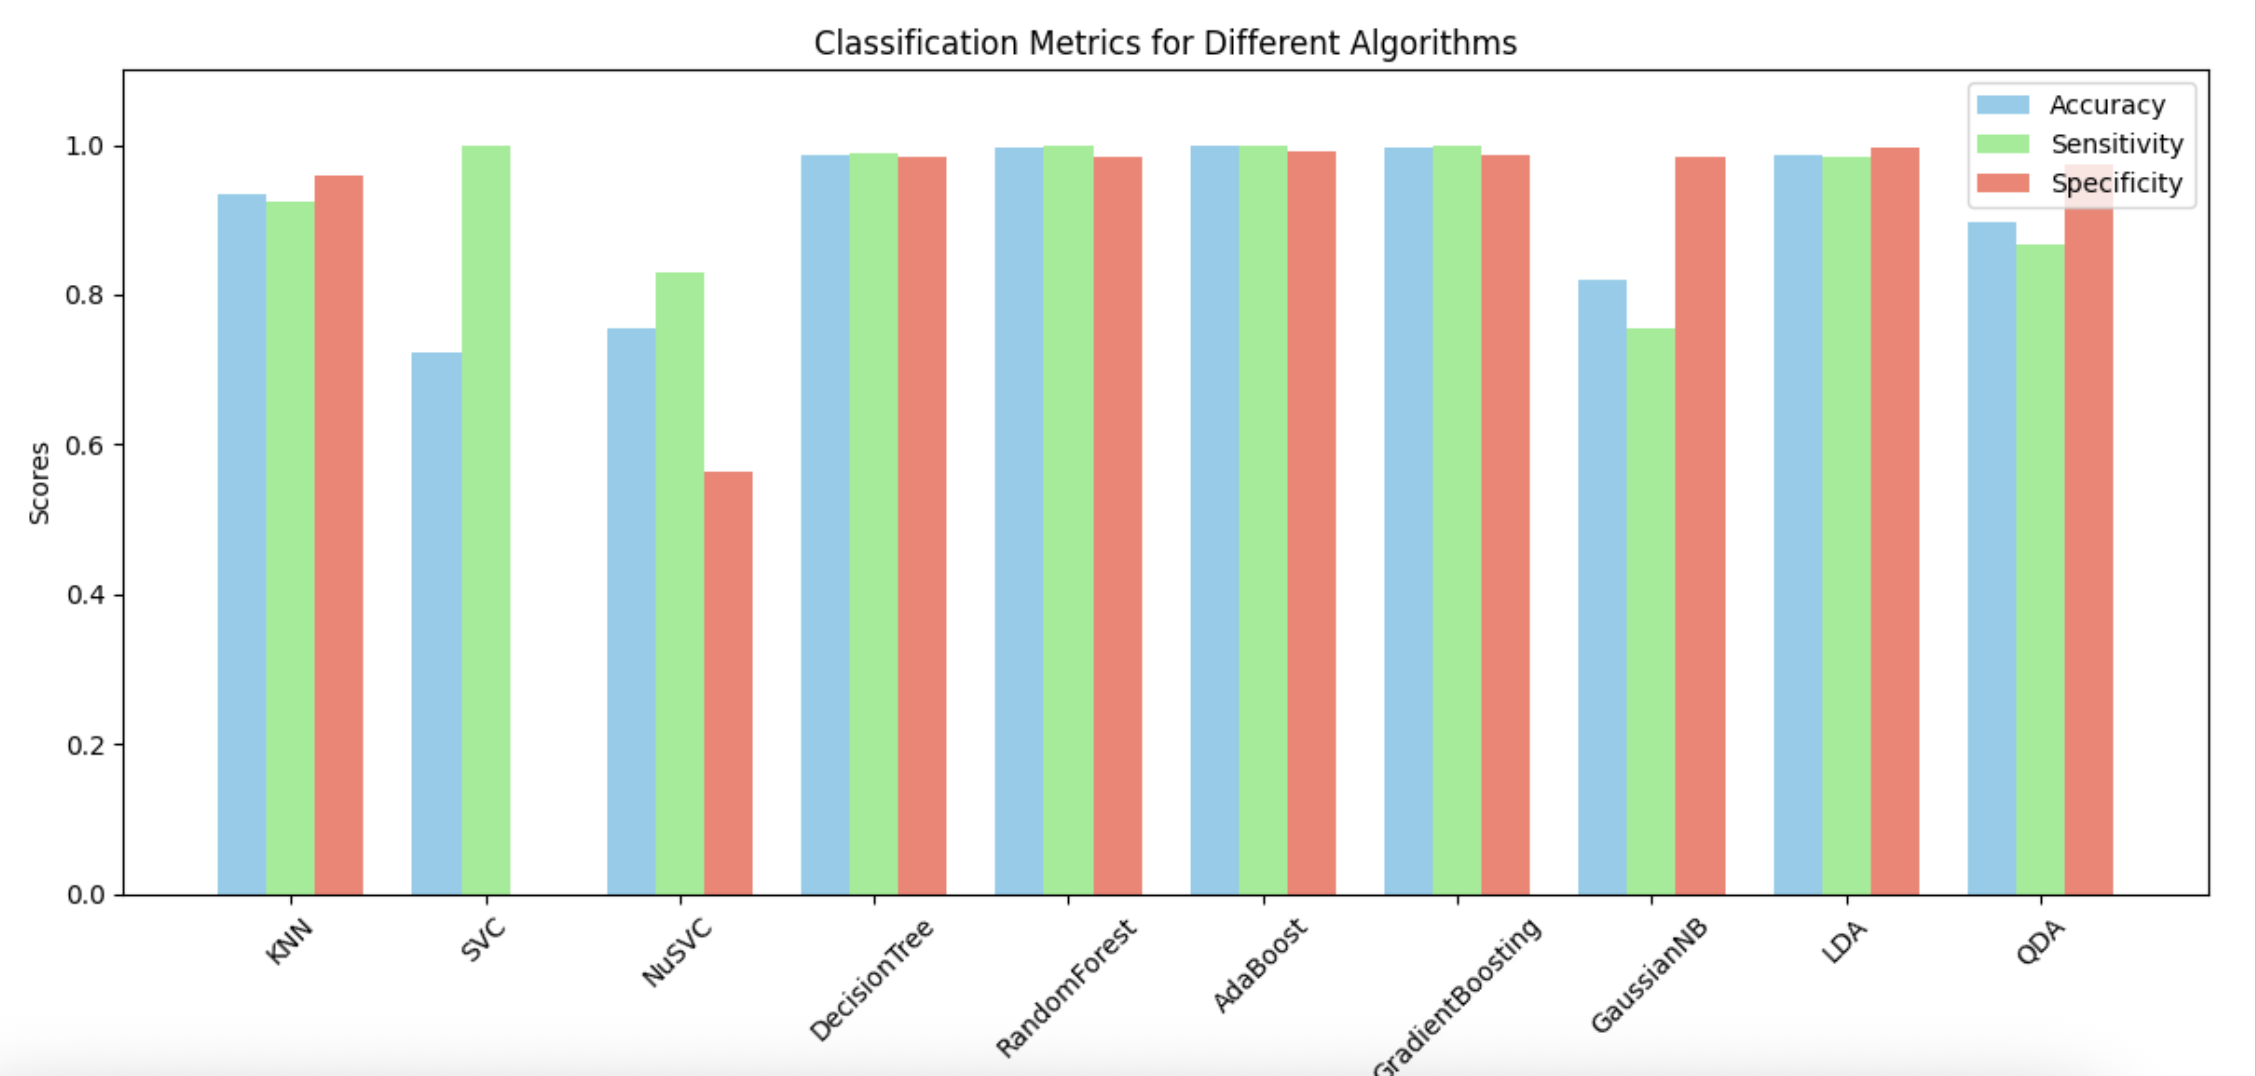
\includegraphics[scale=0.18]{imgs/ClassificationAlgorithms}
\caption{Comparasion of Algorithms}
\label{classificationalgorithms}
\end{figure}

\subsubsection{Feature Importance and Interpretation}
\label{resultsfeatureimportanceandinterpretation}

The top 10 features, shown in Figure~\ref{classificationalgorithms}, identified by each model revealed both lexical and structural indicators of phishing. Across classifiers, features such as Number diversity, Words of length 16, Use of upper case, and Words of length 1 consistently appeared among the most important, highlighting their strong discriminatory power.

In Logistic Regression, the sign of the coefficients provided further interpretability. Positive coefficients (e.g., Number diversity, Use of numbers) indicated a higher likelihood of an email being phishing, reflecting the frequent use of numbers and unusual content in phishing messages. Negative coefficients (e.g., pronouns frequency, Words of length 3) were associated with legitimate emails, capturing normal conversational patterns.

Tree-based models corroborated these findings, emphasizing the predictive importance of structural and lexical features such as punctuation usage, word length distributions, and capitalization patterns. By combining insights from both coefficient signs and feature importance rankings, we identified a set of robust, actionable features that effectively distinguish phishing from legitimate emails (Figure~\ref{boxplots}).

\begin{figure}[h]
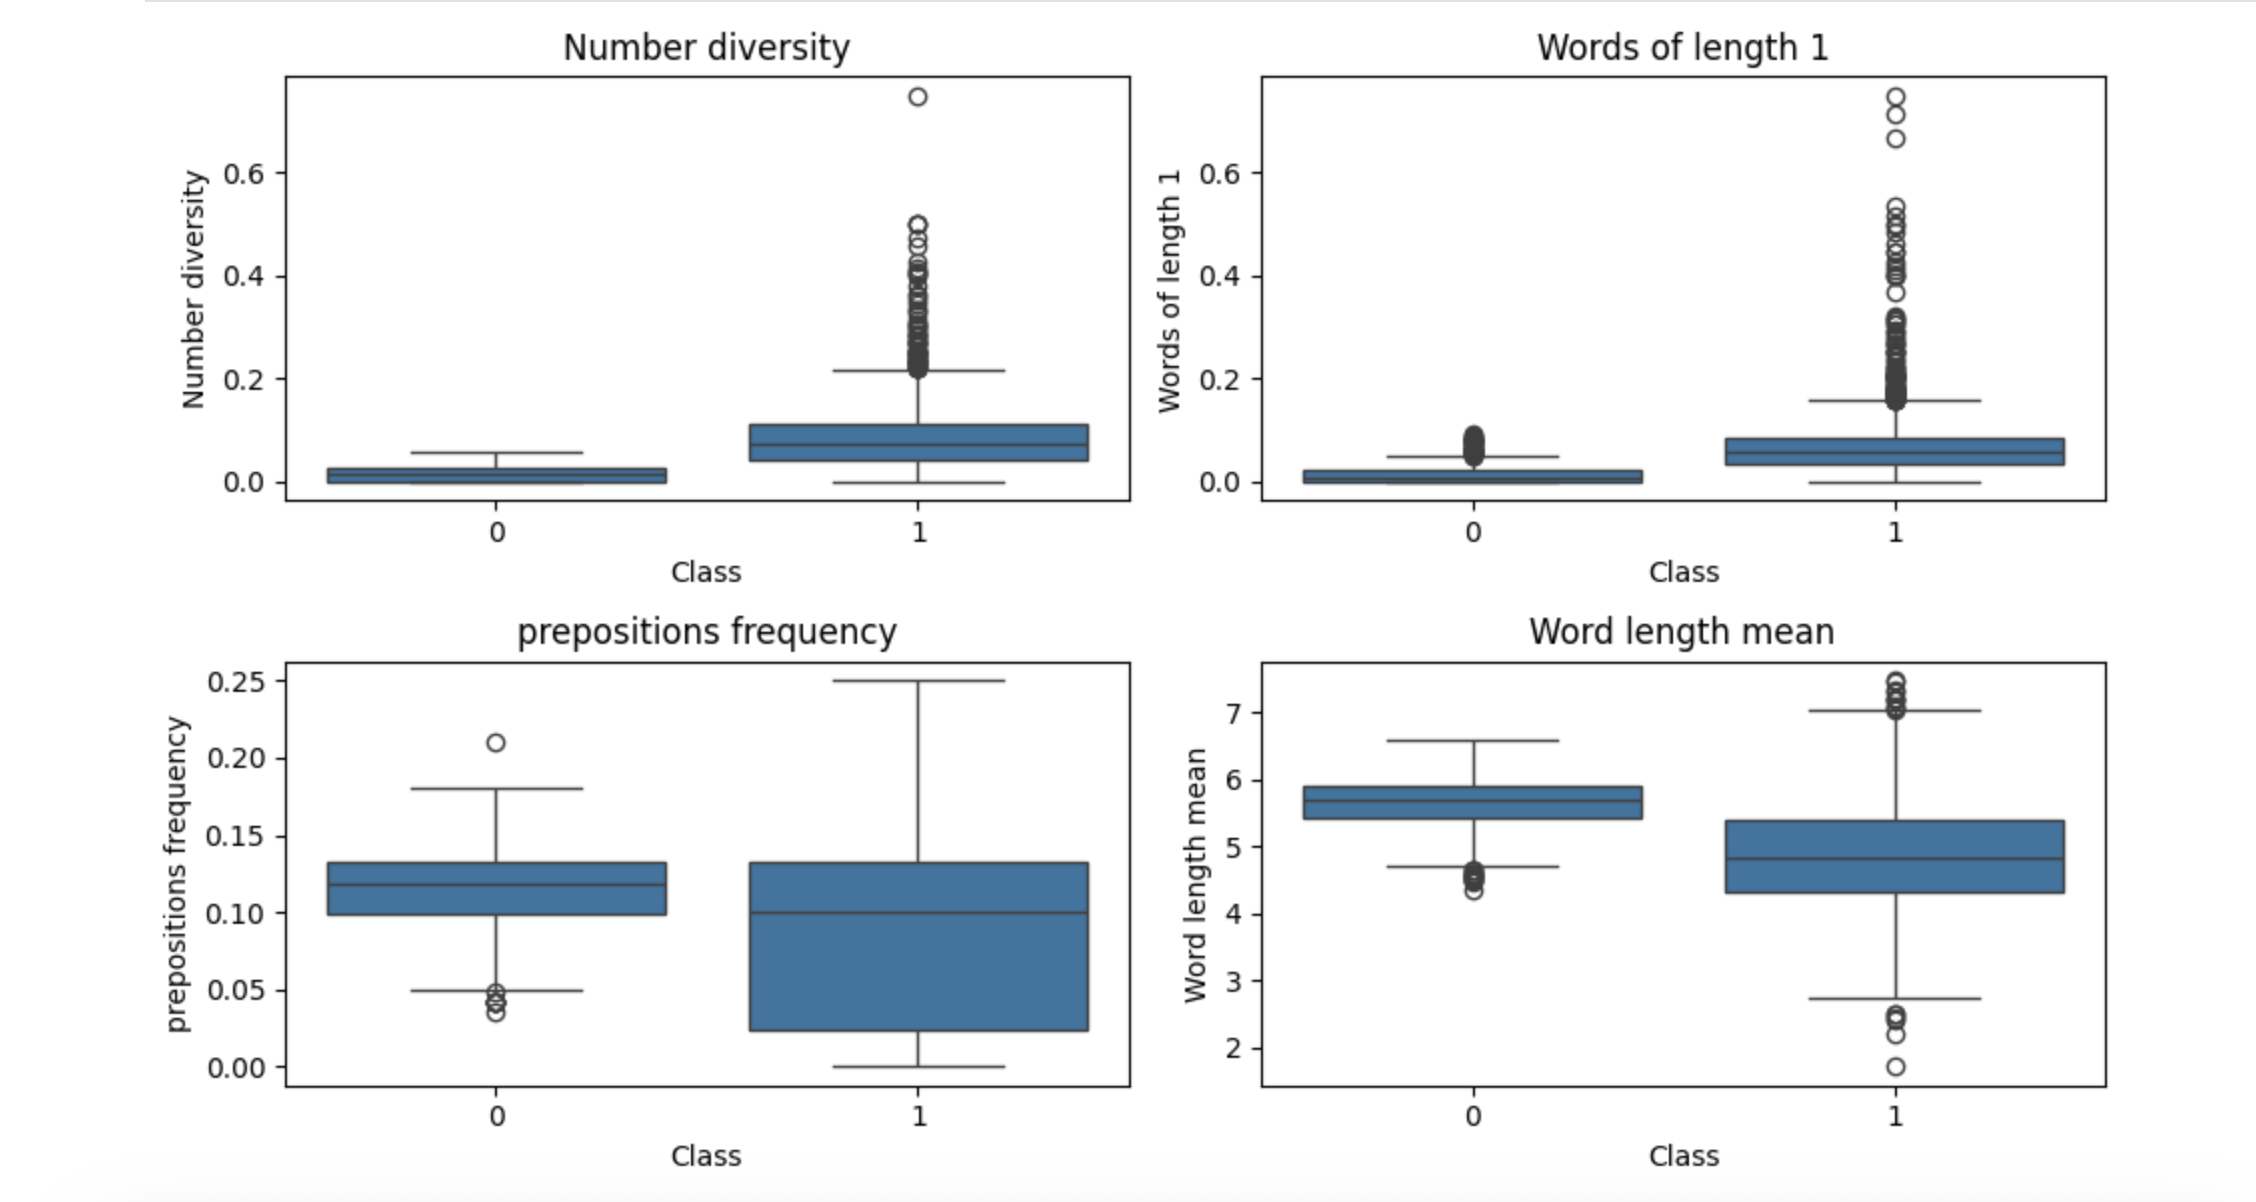
\includegraphics[scale=0.19]{imgs/BoxPlots}
\caption{Features and Box Plot}
\label{boxplots}
\end{figure}

\subsubsection{Error Bar Analysis}
\label{resultserrorbaranalysis}

The 5-fold cross-validation with error bars demonstrated that the top five classifiers are highly consistent (Figure~\ref{errorbar}). Small standard deviations indicate that performance is stable across different subsets of data, supporting the reliability of the selected features and models. AdaBoost and Random Forest not only achieve high accuracy but also show minimal variance, reinforcing their suitability for robust phishing detection.

\begin{figure}[h]
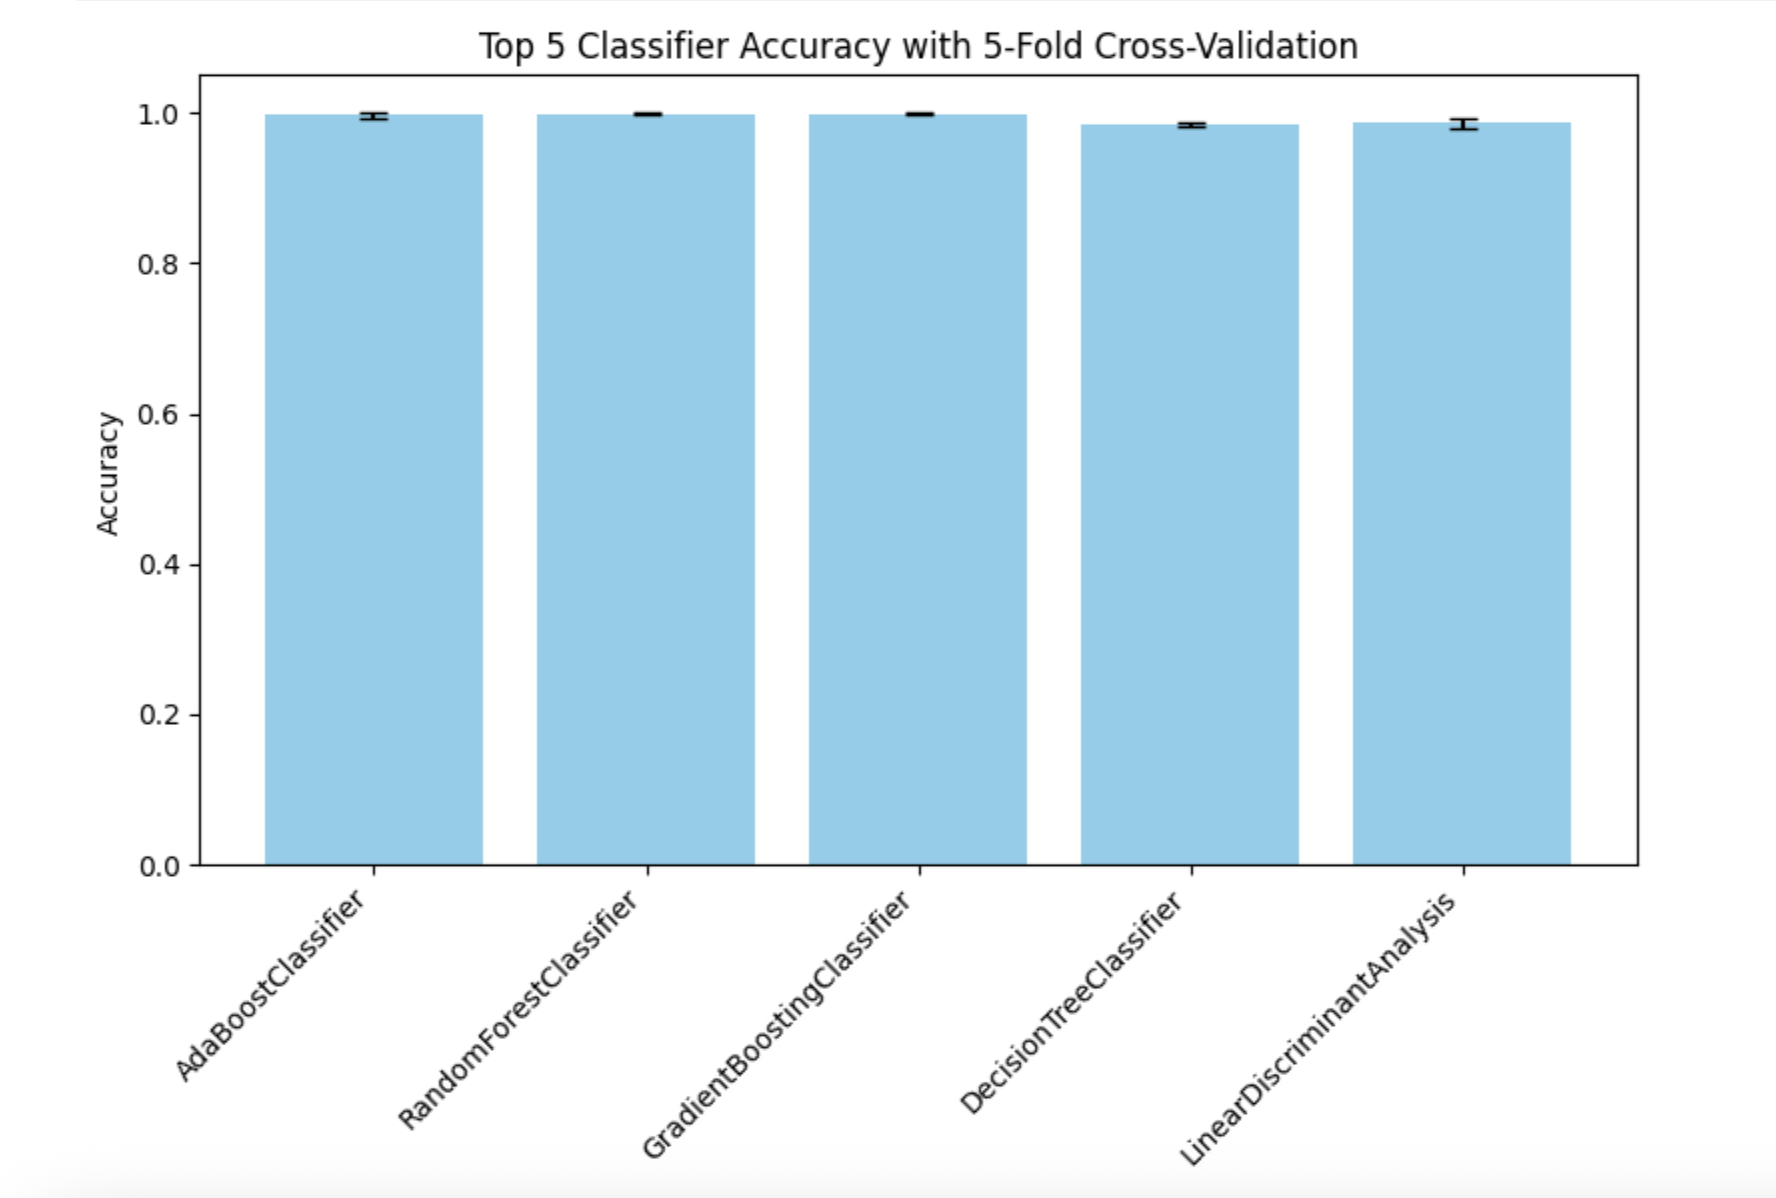
\includegraphics[scale=0.25]{imgs/ErrorBar}
\caption{Top Classifiers With Error}
\label{errorbar}
\end{figure}

\subsubsection{Insights into Linguistic and Structural Cues}
\label{resultsinsightsintolinguisticandstructuralcues}

\begin{itemize}

 \item \textbf{Numeric and Structural Cues}: Phishing emails (Class 0) are characterized by template-like, longer words (e.g., Words of length 16) and repeated structures (Soundex homogeneity), while legitimate emails (Class 1) show higher Number diversity and more frequent short words (Words of length 1). These distinctions highlight the templated nature of phishing emails versus the naturally varied composition of legitimate correspondence.

 \item \textbf{Stylistic and Linguistic Cues}: Legitimate emails exhibit richer linguistic features, including higher Word length mean and Prepositions frequency, reflecting coherent sentence construction. In contrast, phishing emails use repetitive phrasing and template-driven text patterns, aiding automated detection.

 \item \textbf{Formatting and Punctuation Cues}: Phishing emails show moderate punctuation usage and consistent formatting, whereas legitimate emails contain more variable punctuation and higher Quotations number and Punctuation characters ratio, indicating natural language and formatting variability.


\end{itemize}


\subsubsection{Feature-Class Interpretation}
\label{resultsfeatureclassinterpretation}

By comparing class-conditional means, we infer the tendency of features:

\begin{itemize}
 \item \textbf{Positive association with phishing}: Words of length 16, Soundex homogeneity mean/max, Use of upper case.
 \item \textbf{Positive association with legitimate emails}: Number diversity, Words of length 1, Word length mean, Prepositions frequency.
\end{itemize}


\subsubsection{Implications for Detection}
\label{resultsimplicationsfordetection}

These patterns suggest that combining structural, linguistic, and formatting features allows classifiers to effectively distinguish phishing from legitimate emails. Tree-based models naturally leverage these features, while analysis of class-conditional means provides interpretability and actionable insights for email security.

\subsubsection{Email Length Regression Analysis}
\label{resultsemaillengthregressionanalysis}

Phishing emails were significantly shorter than legitimate emails (Figure~\ref{emailslengthanalysis}). A Random Forest regressor accurately predicted email length based on other features (MAE = 10.82; Pearson r = 0.9708, p \textless 0.001), capturing underlying structural patterns. Correlation analysis showed a moderate positive relationship between email length and phishing likelihood (r = 0.205, p \textless 0.001), confirming that shorter emails are more likely phishing. These results reinforce email length as a strong, interpretable feature consistent with observed stylistic differences.

\begin{figure}[h]
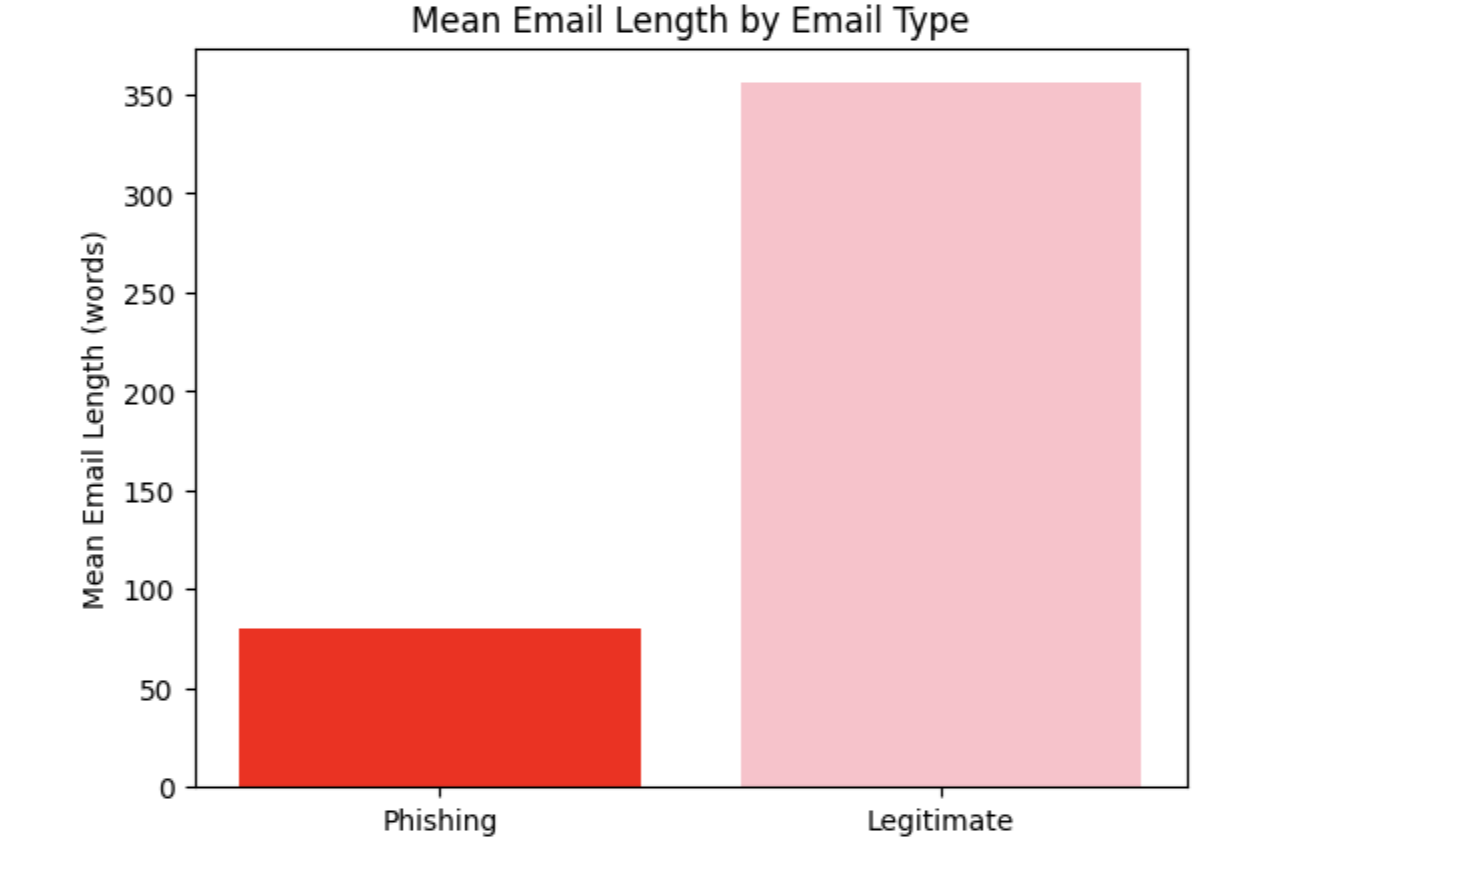
\includegraphics[scale=0.35]{imgs/EmailsLengthAnalysis}
\caption{Mean Length And Class}
\label{emailslengthanalysis}
\end{figure}

\subsection{Outlier Detection}
\label{resultsoutlierdetection}

In order to make the charts easier to understand, charts that are concerned with the subset of the data that contains the legitimate majority are colored in blue for non-outlier detection and red for outlier detection. For charts concerned with the subset of the data containing a majority of phishing emails, green is used for non-outlier detection, and orange is used for outlier detection. An easy way to remember the difference between what information on a given chart is for non-outlier or outlier detection is to ask if it is a cool or warm color. If it is a cool color, blue or green, then it is for non-outliers. If it is a warm color, red or orange, then it is for outliers.

\subsubsection{One Class Support Vector Machines With a Legitimate Email Majority}
\label{resultsocsvmwithalegitimateemailmajority}

First, let’s consider one class support vector machines for a legitimate majority and a phishing minority:

\begin{figure}[h]

\includegraphics[scale=0.47]{imgs/svm_lm_no}
\caption{SVM Non-Outlier Detection Legitimate Majority}
\label{svm_lm_no}
\end{figure}
\newpage

Figure~\ref{svm_lm_no} demonstrates that, in general, the algorithm performs better the higher the gamma, however, this trend does not continue forever, instead plateauing after the 0.20 gamma mark. Additionally, the variation in performance between a given gamma value and its neighbors decreases over time.

It should be noted that the value at 0.00 gamma is 0.00\% due to the algorithm selecting every entry to be an outlier.

\begin{figure}[h]

\includegraphics[scale=0.47]{imgs/svm_lm_o}
\caption{SVM Outlier Detection Legitimate Majority}
\label{svm_lm_o}
\end{figure}

Conversely, the legitimate majority (Figure~\ref{svm_lm_o}) decreases overtime. It plateaus later than the non-outlier detection for one class support vector machine around 0.38 gamma. The variation in performance between a given gamma value and its neighbors decreases over time. The higher early variation leads to 0.04 gamma being the highest performing value for outlier detection at approximately 74\%. This value is higher than the best value local outlier factor’s outlier detection algorithm produced.

It should be noted that the value at 0.00 gamma is 100.00\% due to the algorithm selecting every entry to be an outlier.

\begin{figure}[h]

\includegraphics[scale=0.47]{imgs/svm_lm_noao}
\caption{SVM Combined Legitimate Majority}
\label{svm_lm_noao}
\end{figure}

When looking at one class support vector machine’s performance as a whole (Figure~\ref{svm_lm_noao}), if we consider the values at and around 0.04 gamma, the variation surrounding the gamma is high, but this area is near a sweet spot where both the outlier and non-outlier performance is high. While the non-outlier detection percentage is lower than its maximum at this value, the goal is to find the best outlier detection rate while maintaining at least a reasonable non-outlier detection rate.

For the chart as a whole, the decline in outlier detection and incline of the non-outlier detection rates meet around the 0.10 gamma.

\subsubsection{One Class Support Vector Machines With a Phishing Email Majority}
\label{resultsocsvmwithaphishingemailmajority}

Next, the one class support vector machine was evaluated under a phishing email majority and a legitimate minority:

\begin{figure}[h]

\includegraphics[scale=0.47]{imgs/svm_pm_no}
\caption{SVM Non-Outlier Detection Phishing Majority}
\label{svm_pm_no}
\end{figure}
\newpage

When it comes to a phishing majority, non-outlier detection does not increase or decrease consistently (Figure~\ref{svm_pm_no}), instead it goes through continuous cycles of rising and following. These cycles tend to take longer each time the higher the gamma.

It should be noted that the value at 0.00 gamma is 0.00\% due to the algorithm selecting every entry to be an outlier.

\begin{figure}[h]

\includegraphics[scale=0.47]{imgs/svm_pm_o}
\caption{SVM Outlier Detection Phishing Majority}
\label{svm_pm_o}
\end{figure}

For outlier detection (Figure~\ref{svm_pm_o}), there is no consistent incline or decline, and they increase and decrease cyclically. The range of values encompassing each cycle increases each pass. While the difference between peaks was similar for non-outlier detection, outlier detection has its highest peak early on at 0.05 gamma. It is very close to the peak value for the legitimate majority.

It should be noted that the value at 0.00 gamma is 100.00\% due to the algorithm selecting every entry to be an outlier.

\begin{figure}[h]

\includegraphics[scale=0.47]{imgs/svm_pm_noao}
\caption{SVM Combined Phishing Majority}
\label{svm_pm_noao}
\end{figure}
\newpage

Together we can see that the peaks of the non-outlier performance is offset from the outlier’s performance peaks (Figure~\ref{svm_pm_noao}). When one is at its peak, the other is on a decline. Since the phishing majority looks for legitimate outliers and the best gamma for outlier detection on the phishing majority was 0.05 gamma, it agrees with the prior section's estimation.

\subsubsection{Local Outlier Factor With a Legitimate Email Majority}
\label{resultslofwithalegitimateemailmajority}

Let’s now consider the local outlier factor algorithm on a legitimate majority and phishing minority:

\begin{figure}[h]

\includegraphics[scale=0.47]{imgs/lof_lm_no}
\caption{LOF Non-Outlier Detection Legitimate Majority}
\label{lof_lm_no}
\end{figure}

For non-outlier detection (Figure~\ref{lof_lm_no}), a lower number of neighbors produces the best result with a very shallow decline as the number of neighbors increases. The best value appears around 6 neighbors.

\begin{figure}[h]

\includegraphics[scale=0.47]{imgs/lof_lm_o}
\caption{LOF Outlier Detection Legitimate Majority}
\label{lof_lm_o}
\end{figure}
\newpage

For outlier detection (Figure~\ref{lof_lm_o}), outcomes remain low and decrease over time, eventually to zero shortly after 60 neighbors. This makes sense as there are 50 phishing emails, and if the number of neighbors is higher, it will invariably include legitimate emails that will decrease the accuracy. The highest detection rate was when only a single neighbor was considered, however, it is considerably lower than one class support vector machine’s maximum value.

\begin{figure}[h]

\includegraphics[scale=0.47]{imgs/lof_lm_noao}
\caption{LOF Combined Legitimate Majority}
\label{lof_lm_noao}
\end{figure}

Together (Figure~\ref{lof_lm_noao}), we see that while the non-outlier detection rate is consistently high, the outlier detection rate is very low. The algorithm is “safe” this way, including few non-outliers, but it selects few of the actual targeted outliers.

\subsubsection{Local Outlier Factor With a Phishing Email Majority}
\label{resultslofwithaphishingemailmajority}

Finally, the local outlier factor algorithm was evaluated under a phishing email majority and a legitimate minority:

\begin{figure}[h]

\includegraphics[scale=0.47]{imgs/lof_pm_no}
\caption{LOF Non-Outlier Detection Phishing Majority}
\label{lof_pm_no}
\end{figure}

The non-outlier detection (Figure~\ref{lof_pm_no}) rates for a phishing majority is very similar to the non-outlier detection rates for a legitimate majority, however, instead of decreasing slightly, it increases slightly. 98 neighbors performed the highest around approximately 97\%.

\begin{figure}[h]

\includegraphics[scale=0.47]{imgs/lof_pm_o}
\caption{LOF Outlier Detection Phishing Majority}
\label{lof_pm_o}
\end{figure}

The outlier detection rate for a phishing majority is also similar to the non-outlier detection rates for a legitimate majority (Figure~\ref{lof_pm_o}). It increases in the beginning, but then decreases before leveling off at 80\% around 59 neighbors. The highest value occurs around 16 neighbors at approximately 89\%.

\begin{figure}[h]

\includegraphics[scale=0.47]{imgs/lof_pm_noao}
\caption{LOF Combined Phishing Majority}
\label{lof_pm_noao}
\end{figure}
\newpage

Together (Figure~\ref{lof_pm_noao}), the best outlier detection rate around 16 neighbors is the best candidate. While the phishing majority outcome appears to be a solid contender against the 0.04 gamma option from the one class support vector machine algorithm, the difference between the phishing majority’s outlier detection rate and the legitimate majority’s outlier detection rate for the local outlier factor algorithm demonstrates that the algorithm performs worse under conditions where there are less phishing emails compared to legitimate emails while the one class support vector machine algorithm performs more consistently while agreeing on an optimal value.

\subsubsection{Evaluating the Best Outlier Algorithm Settings}
\label{resultsevaluatingthebestoutlieralgorithmsettings}

Given this optimal solution of one class support vector machine with a 0.04 gamma, we can run it against the entire dataset in order to determine performance (Table~\ref{svmtable}).

\newpage
\textbf{One Class Support Vector Machine (0.04 Gamma)::}

\begin{table}[h]
        \caption{One Class Support Vector Machine (0.04 Gamma) Results}
\begin{tabular}{l|l|l|}
\cline{2-3}
                                                & Legitimate     & Phishing      \\ \hline
\multicolumn{1}{|l|}{Identified as Non-Outlier} & 61.28\% (1220) & 48.32\% (418) \\ \hline
\multicolumn{1}{|l|}{Identified as Outlier}     & 38.72\% (771)  & 51.68\% (447) \\ \hline
\end{tabular}
\label{svmtable}
\end{table}

\textbf{Local Outlier Factor (16 Neighbors)::}

\begin{table}[htp]
\caption{Local Outlier Factor (16 Neighbors) Results}
\begin{tabular}{l|l|l|}
\cline{2-3}
                                                & Legitimate     & Phishing      \\ \hline
\multicolumn{1}{|l|}{Identified as Non-Outlier} & 85.83\% (1709) & 96.07\% (831) \\ \hline
\multicolumn{1}{|l|}{Identified as Outlier}     & 14.16\% (282)  & 3.93\% (34)   \\ \hline
\end{tabular}
\label{loftable}
\end{table}

When it comes to detecting phishing emails, the one class support vector machine at 0.04 gamma performed much better (51.68\%) than the local outlier factor algorithm with 16 neighbors (3.93\%) (Table~\ref{loftable}).

However, the local outlier factor algorithm performed better at labelling legitimate emails as non-outliers (85.83\%) compared to one class support vector machine’s performance (61.28\%).

This follows the expected outcome from earlier in the section where the local outlier factor algorithm would be better at minimizing false positives while the one class support vector machine algorithm performed much better when labelling true positives.

This outcome means that the immediate neighbors for phishing emails do not allow us to make an immediate determination unless they are in a clear majority. In our data, they are the minority as they are less than a third of the number entries.

Since support vector machines work under the assumption that most data is normal \citep{bhakta}, this higher performance may indicate that phishing emails can be represented better by their deviation rather than by their neighboring elements. Again, this is assuming that the evaluated data resembles our data, that is, it is when phishing data is in the minority.

\section{Conclusion}
\label{conclusion}


%This section is the analysis of the results presented in the Results section, and should describe the conclusion of your work. It should describe the meaning of the results, the advantages of your work compared to existing knowledge, and information that we can learn from the results.

%It should also discuss the weaknesses of the analysis, and things we cannot conclude from our results. You can also use the Conclusion section to discuss potential uses of the work, and ideas for future work.

This study demonstrates that phishing emails can be effectively distinguished from legitimate emails using a combination of structural, linguistic, and formatting features. Statistical analysis revealed that phishing emails are generally shorter, employ template-driven text patterns, and exhibit distinct numeric and punctuation usage compared to legitimate messages. Frequency-domain features further highlighted systematic differences in textual patterns, reinforcing the presence of consistent stylistic cues in phishing emails.

Machine learning classifiers, particularly ensemble and tree-based models such as Random Forest, AdaBoost, and Gradient Boosting, achieved high and balanced accuracy (\>99\%) in detecting both phishing and legitimate emails. Feature importance analysis revealed that attributes such as Number diversity, word length distributions, use of uppercase letters, and Soundex homogeneity are highly predictive, providing interpretable insights into the structural and linguistic characteristics of phishing messages. Cross-validation confirmed the robustness and stability of these models, emphasizing their reliability for real-world applications.

Additionally, email length was found to be a strong, interpretable feature, with shorter emails being more likely phishing. Regression analysis confirmed that this feature captures underlying structural differences, supporting the overall classification framework.
Overall, the findings indicate that carefully selected features combined with robust machine learning models enable highly accurate, interpretable, and reliable phishing email detection. These results have practical implications for automated email security systems, providing actionable insights for designing classifiers that can effectively mitigate phishing threats.

For outlier detection, one class support vector machines perform better when detecting phishing emails compared to local outlier factor’s performance. One class support vector machine’s ability to detect phishing emails over the entire dataset at 51.68\% is not better than random selection, however, it avoids selecting legitimate emails as outliers better than random selection at 61.28\% successful identification. Since one class support vector machine’s outlier detection performance is much higher than local outlier factor’s performance, it may be the case that considering the normalcy of the data is more valuable than considering the neighbors of any individual entry.

The datasets we utilized, compared to the velocity and scale of a real world application is severely limited. As such, our conclusions are potentially limited in scope and application. The benefit of focusing on shallow learning techniques means that we do, however, gain some insight on where to look in the future. Future work should consider these algorithms and findings on a large scale. Using massive datasets and datasets with a high velocity could allow these findings to be tested in an environment that reflects a real world scenario.

\section*{Acknowledgments}

%List here any person who assisted you in your work. Receiving help from others is basically allowed (and sometimes even encouraged) in this course, but please consult with me before asking for someone else’s help.

\begin{itemize}
 \item Dr. Shamir
 \subitem We would like to thank Dr. Shamir for his guidance on data sources and methodology.
\end{itemize}


\section*{Author contribution}

%Briefly describe the contribution of each author to the preparation of the data, design of the experiments, analysis of the results, and the writing of the paper.

\begin{itemize}
 \item Saloni Parkash
 \subitem Writing: Abstract
 \subitem Feature Selection
 \subitem Writing: Methods - Feature Selection
 \subitem Writing: Results - Feature Selection
 \item Sierra Hawbaker
 \subitem Data Sanitization and Random Sampling of Data
 \subitem Background Research
 \subitem Outlier Detection
 \subitem Conversion of Document to Latex
 \subitem Writing: Methods - Outlier Detection
 \subitem Writing: Results - Outlier Detection
 \item Shared
 \subitem Writing: Introduction
 \subitem Writing: Data
 \subitem Writing: Conclusion
 \subitem Coordination of Tasks
\end{itemize}


\bibliographystyle{apalike}

\bibliography{main}

\end{document}



